% !TEX root = ../main.tex
% !TEX program = XeLaTeX
% !TEX encoding = UTF-8 Unicode

\date{2018년 3월 21일}

\begin{frontmatter}
\title{빠꼬어}
\author{김성}
\address{한국외국어대학교 베트남어과}
\begin{abstract}
Alves, Mark J. (2006). A grammar of Pacoh: a Mon-Khmer language of the central highlands of Vietnam. Pacific Linguistics, Research School of Pacific and Asian Studies, The Australian National University, 26--53.
\end{abstract}
\end{frontmatter}

%%%%%

\section*{발제 범위 분배}
\begin{table}[h]
\begin{center}
\def\arraystretch{1.5}
\begin{tabular}{>{\sffamily}ccccl}
\hline
	&\itshape 발제자	&\itshape 발제 범위		
	&\itshape 페이지	&\itshape 내용\\
\hline
1 & 김성 & Ch. 1-2 & pp. 1-25 & 서론, 음운론 \\
2 & 김성 & Ch. 3-6 & pp. 27-53 & 형태론, 기본 구 구조 개괄, 부사, 접속사 \\
3 & & Ch. 7 & pp. 54-77 & 명사 \\
4 & & Ch. 8-10 & pp. 79-103 & 전치사, 문장 소사, 기본 동사 \\
5 & & Ch. 11 & pp. 106-111 & 보조 동사, SVC, VCT 동사 \\
\hline
\end{tabular}
\end{center}
\end{table}

\section*{Register에 따른 최소대립쌍}

\begin{center}
\textbf{Minimal pairs of Pacoh plain and creaky vowels} 

\begin{tabular}{l|lll}
\textbf{phonation} & \textbf{Vowel} & \textbf{Example} & \textbf{Gloss} \\
\hline
plain & o & koh & that/there \\
creaky & o̰ & ko̰h & mountain \\
plain & e & ceːt & pen \\
creaky & ḛ & cḛːt & die \\
plain & uə & puəh & make traps \\
creaky & ṵə & pṵəh & white
\end{tabular} 
\end{center}
\hfill [Alves, 2000:34]

\setcounter{section}{2}

\section{형태론}
\begin{itemize}
\item 접사와 중첩어는 유추적 패턴(analogical patterns)이라는 측면에서 다루어진다. 원어와 파생된 형태를 보여주는 유추적 세트(analogical sets)가 제공된다.

\item /C/는 어근의 음절초 자음에서 베껴진 자음을, /V/는 어근에서 베껴진 모음을 나타낸다.
\item 본 섹션 전체에서 접사는 괄호로 구별하여 표시한다. 이는 접사의 실제 이형태적인 변이형이 아니라 추상적인 음운론적 형태를 나타내기 위한 것이다.
\end{itemize}

27-28 표24.

주음절에서 받아오는 음소가 인상적이다. 주음절에서 받아오는 음소로만 구성된 접두사도 있다.(CV-)

접사의 생산성은 크게 셋으로 나뉘는데 
\begin{itemize}
\item 가장 생산적인 접사에는 [par1-] `X하는 행동' 와 [tar-] `서로 X하다' 가 있다. 이들은 새로운 단어를 자유롭게 형성해 낸다.
\item{ [ta-] `본의 아니게 X하다', [pa-] `X하게 하다', [CV-] `일반적으로 X하다(to X in general)' 등의 접사는 최소한의 생산성을 보인다.}
\item{ [-an-], [pi-] `X가 되게 하다', [par2-] `서로 X하게 하다', [ti-] `X당하다', [Ca-] `완전히 X하다' 등의 접사는 기본적으로 화석화된 잔재이다.}
\item 중첩어(표24에서는 `X하는 척 하다') 에 대해서는 생산성 검증이 되지 않았는데, 상당한 수의 중첩 형태가 있으므로 최소한 얼마 정도는 생산적일 것으로 보인다.
\item 이상의 통계는 30년 전의 것이고 저자가 최근에 접촉한 화자들은 일부 접사를 알아보았지만 일부는 알아보지 못했다. 일부 접사는 소실되고 있을 가능성이 있다.
\end{itemize}

\subsection{명사 형태론}
\subsubsection{보통 명사}
빠꼬어에는 동사로부터 파생되어 접요사 [-an-]이나 그 다양한 이형태를 음절 접연부에 포함하는 2음절 명사의 그룹이 있다. (역사적으로는 원시 몬·크메르어의 도구(instrumental) 접요사 [-rn-]를 반영하는 것이고 빠꼬어에는 그 화석화된 잔재가 몇 가지 남아 있지만, 이 문법서에서는 공시적 기술을 위해 이 접요사 하나만을 소개한다.) 
이 부분열(접요사 부분)에 속하는 자음은 후행하는 자음의 조음 위치에 부분적으로 동화되거나 후행하는 /l/ 또는 /r/ 분절음에 완전히 동화된다. 그러나 이는 절대적인 것이 아니라 경향성이며 예외가 존재한다. 접요사 내의 모음은 닫힌 전음절에서 언제나 음성적으로 슈와로 실현된다. 

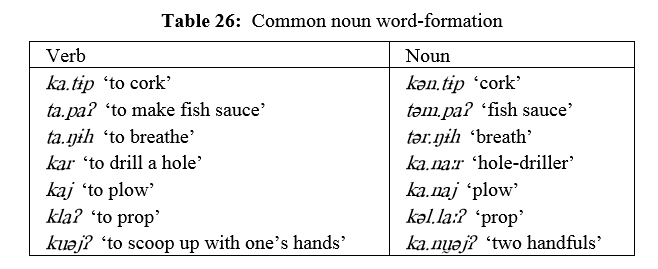
\includegraphics{Pacoh/src/PacohTable26.png}	

%가산, 불가산 여부나 어떤 단위명사가 의미적으로 연결되는지 등의 의미적 자질에 따라 통사적으로 분포적인 자질이 있음.??

\begin{itemize}
\item \textbf{S6}
\gll pḛːh kən.nɔh kɔh ʃḛːc bṵəjʔ\\
\itshape{take} \itshape{cutter} \itshape{cut} \itshape{meat} \itshape{fish} \\
`Take the cutter and cut the fish meat'
\end{itemize}

\subsubsection{친족어, 동물 이름 어휘 형성}
\begin{itemize}
\item 대부분의 빠꼬어 친족어는 전음절 [ʔa-]로 시작한다. (브루어, 까뚜어, 따오이어 등 다른 까뚜어군 언어들과 마찬가지이다.)
\item 이러한 친족어 발전 과정은 화석화된 것으로 보인다. [ʔa-]가 없는 유사한 패러다임은 찾아볼 수 없다.
\end{itemize}

표27 (30페이지) 은 대표적인 예만을 나타낸 것이다.

\begin{itemize}
\item 빠꼬인들의 환경에 많이 사는 동물을 가리키는 말을 포함해 많은 수의 빠꼬어 동물 지칭어도 또한 전음절 [ʔa-]로 시작한다.
\end{itemize}

표28은 ND\&P의 빠꼬어--따오이어--베트남어 사전의 40개 가량 되는 표제어 중 일부.

\subsubsection{대명사 형태론}
접사로 연결된 대명사와 지시사.
인칭 3개와 수 3개로 9개의 기본 대명사 세트가 구성된다. 거기에 여격 세트와 소유격 세트가 추가되어 세 배가 된다.

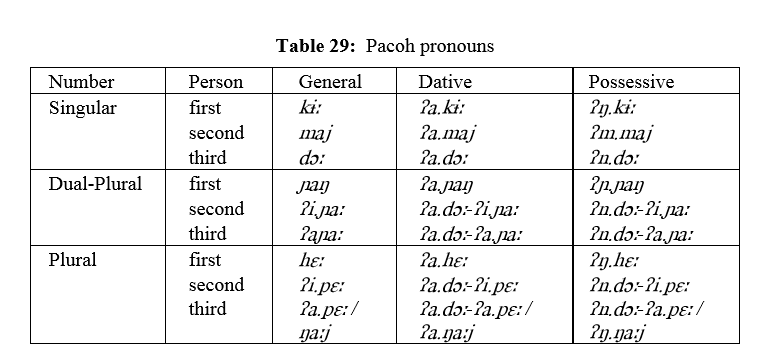
\includegraphics{Pacoh/src/PacohTable29.png}

\begin{itemize}
\item 단수가 아닌 대명사 중 이인칭 대명사는 전음절 [ʔi-], 삼인칭 대명사는 전음절 [ʔa-]가 나타난다.
\item 여격 대명사는 접두사 [ʔa-]를 공유한다. 
\item 소유격 대명사는 조음점이 같은(homorganic) 비음 접두사가 나타난다.
\item 이음절 대명사는 삼인칭 대명사를 특수 접사로 받아들인다.(? `Bisyllabic pronouns take third person pronouns as special affixes')
\end{itemize}

지시대명사는 전반적으로 유사한 운율적, 음운론적 형태를 갖추었다.
\begin{itemize}
\item 이음절어이고
\item 조음점이 같은 비음 전음절을 갖추며
\item 어말에 [h] 자음을 갖는다.
\end{itemize}
중간 거리와(medial) 먼 거리(distal) 지시대명사는 모음의 장단에서 차이가 나타난다. 전자가 단모음, 후자가 장모음을 갖는다. 빠꼬어의 가까운 친족어인 브루어(Bru)에서는 지시대명사에서 모음의 장단과 지시 대상의 거리의 연관성이 더 복잡하게 나타난다.

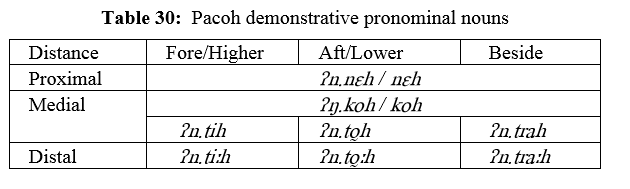
\includegraphics{Pacoh/src/PacohTable30.png}

\subsubsection{어휘적 합성어}
명사-명사 연속을 늘 두 단어의 연속으로 보기에는 분석 상 다양한 어려움이 따르므로 한 단어로 본다. Ng and Starosta (1996) 참조.

S8에서 `Vietnamese'를 따로 뗄 수 없고 추가적인 수식어는 그 바깥에 붙는다.

이러한 접근은 빠꼬어에서 의미적으로 일반화된 명사를 분석하는 데 중요하다.
S9, S10.
이러한 명사도 절-포함(clause-incorporation)에 사용되는 음운론적 재료를 제공한다.(3.3.1.)

\subsubsection{시간-어휘 형태론}
1에서 10까지 날이나 해의 수로 과거 또는 미래를 나타내는 굉장히 분명한 체계가 발달되어 있다. 까뚜어군 등 다양한 언어들에서 비슷한 현상이 나타난다.
(1) 과거의 날, (2) 과거의 해, (3) 미래의 날, (4) 미래의 해에 대한 네 가지의 접사 유형이 있다. 이러한 접사는 3이상의 숫자를 나타내는 시간 명사에는 완전한 규칙성을 보이며 결합되지만 2를 나타내는 시간 명사에서는 약간의 음운론적 변이가 나타난다.
모든 단어가 `날' 이나 `해'를 나타나는 단어를 갖고 있으며 대부분의 단어가 그 가리키는 숫자에 따라 3에서 10을 나타내는 수사와 운(rhyme)이 같다. 과거의 날이나 해를 나타내는 단어에는 [-ʔn.tr-]가 붙고 미래의 날을 나타내는 단어에는 [pər], 미래의 해를 나타내는 단어에는 [-ku.m-] 이 붙는다.

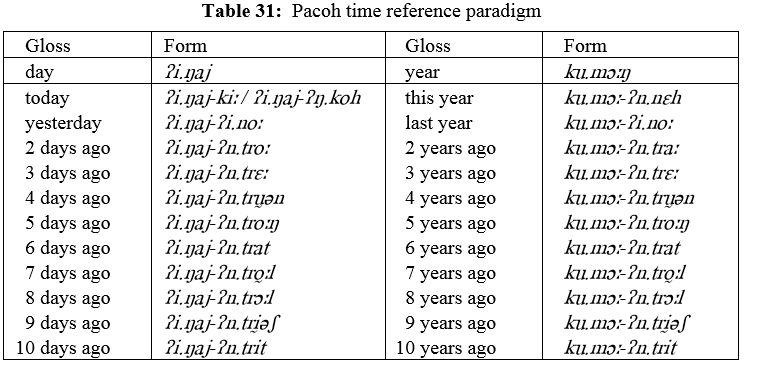
\includegraphics{Pacoh/src/PacohTable31-1.png}

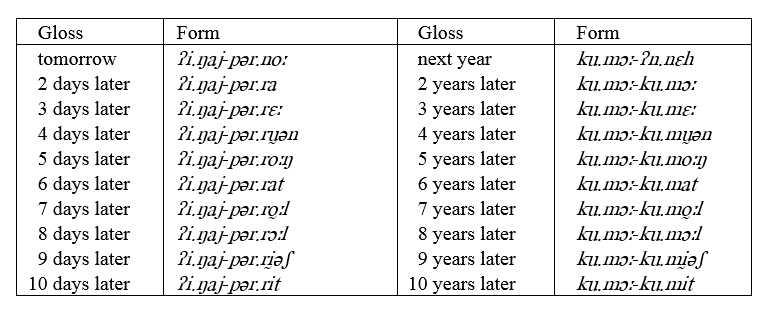
\includegraphics{Pacoh/src/PacohTable31-2.png}

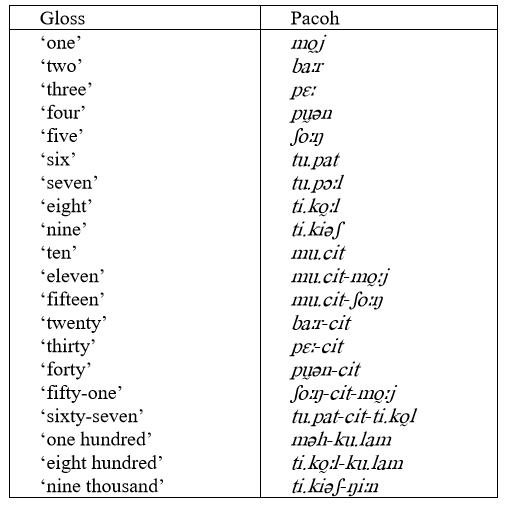
\includegraphics{Pacoh/src/Pacohnumerals.png}

\subsection{동사 형태론}
%주어와 목적어의 분포를 고려할 때 빠꼬어 동사 형태론에서 몇 가지 의미적 기능은 통사적으로 더 영향력 있다.
\subsubsection{사역 동사}
다른 몬·크메르어파 언어들에서도 나타나는 동사 그룹이다. [pa-]라는 일반형을 갖는 전음절을 공유하고 그 목적어로 하여금 어떠한 행동을 하게 하는 의미적 기능을 갖는다.
표32. 부분적 예시. [pa-] 외에 [ta-], [ʔa-]가 보임.

어근의 통사적 동사 부류는 상관 없지만 대부분은 일음절 동사이다. 음운론적 기본형(base)는 음운론적으로 조건지어졌든지 아니든지 몇 가지 음운론적 변이형이 나타난다. 음절초 [p]외에 음절초 [t]나 [ʔ]도 나타나며 이는 어휘적 파생의 불규칙성 뿐만 아니라 이러한 형태가 빠꼬어에서 오래 존재해 왔을 가능성을 나타내는 것이기도 하다.

S11 깨물게 하다 잠자게 하다

빠꼬어 사역동사는 다양한 논항과 보어를 취하는 다양한 종류의 동사에서 나타난다.
S12, S13, S14

\subsubsection{대명사 접두사 [ʔu-], [ʔi-]가 나타나는 동사}
빠꼬어에서 접두사 [ʔu-] 나 [ʔi-]를 갖는 동사는
명시적인 주어 명사를 취하지 않을 수 있다. ([ʔu-], [ʔi-]를 접두사 대신 접어(clitics), 즉 음운론적으로 결합되어 있지만 통사론적으로는 자유로운 형태로 볼 수도 있다. 그러나 이 문제에 대해 논하기에는 자료가 부족하다.)
이 접사들의 의미·통사론적, 화용론적 기능이나 생산성은 아직 완전히 밝혀지지 않았다.

S. Watson (1964:88) 에서는 [ʔu-] 동사가 나타나면 3인칭 대명사를 대체한다고 언급했다. 결과적인 형태는 S16에서처럼 사람이 주어인 것으로만 해석된다.
\begin{itemize}
\item \textbf{S15}
\gll ʔu.toːŋ nɨːm məh naʔ ʔa.caːj\\
\itshape{3s-say} \itshape{only} \itshape{one} \textsc{unit} \itshape{brother} \\
`He said he has only one brother.'

\item \textbf{S16}

\begin{tabular}{lcl}
poːk {\itshape{`go'}} & : & ʔu.poːk {\itshape{`He/she goes'}} :: \\
dɔːk {\itshape{`read'}} & : & ʔu.dɔːk {\itshape{`He/she reads'}}
\end{tabular}
\end{itemize}

전음절 [ʔi-]는 부정인칭을 나타낸다. R. Watson (1966a:168) 에서는 이러한 전음절을 `subject fillers'라고 불렀다. S17(a)와 같은 용법도 가능하지만 S17(b)에서처럼 상태동사를 따라 나타나는 경우가 많다. S18에서처럼 피동 표지 대신 주제·논평(topic-comment) 구조에서 나타나기도 한다. (수동태가 없는 언어라는 개념은 적어도 전통적인 유럽의 관점에서는 논란의 여지가 있다. Alves (1998) 에 베트남어에 대한 그러한 주장이 담겨 있다.)

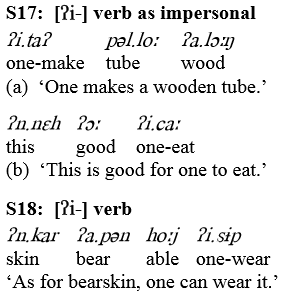
\includegraphics{Pacoh/src/PacohS17.png}

\subsubsection{복수 상태 동사}

전음절 [Ca-] (`C'는 어근 형태의 음절초 자음에서 베껴진 자음) 는 (복수 표지가 명시되어 있든 그렇지 않든) 의미 자질이 (주로 무생물 명사인) 복수 주어를 가리킨다는 것을 나타내기 위해 
일음절 상태동사와 결합한다.

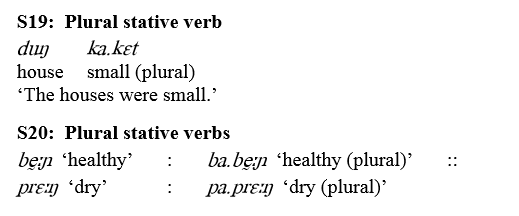
\includegraphics{Pacoh/src/PacohS19.png}

\subsubsection{상호 동사}
[tər-] (또는 유사한 음운론적 형태 [ʔr-]나 [kər-]) 는 특정 동사에서 상호성 표지이다. [pər-] 같은 경우는 사역동사이면서 상호동사인 경우 나타난다.

\subsubsection{결과 부사}
접두사 [ʔa-]가 일음절 동사 어근과 결합해 결과적인 의미가 있는 부사를 만든다.

\subsection{중첩}
몬·크메르어에서의 중첩어는 주로 능동 상태 동사에서 나타나지만 명사나 부사에서도 나타난다. 

빠꼬어 중첩어로 표현되는 공통적인 의미장에는 의미적으로 굉장히 구체적이어서 정확히 번역하기 어려운 것들이 포함된다.
\begin{itemize}
\item 물리적 느낌
\item 냄새
\item 복잡하거나 엉망인 상황
\item 의미적으로 전문적인 행동
\end{itemize}

접근 가능한 98개 중첩어 데이터 중 9개가 부사, 20개가 명사, 25개가 비 상태동사, 42개가 상태동사이다.

\subsubsection{절 결합적인 어휘 형성}
이 어휘 형성 과정은 문장이나 문장의 부분으로부터 취한 음운론적 소재를 중첩에 수반시킨다. 일반적으로, S23(a)와 (b)에서 각각 그렇듯, 중첩어휘와 일반화된 명사를 수반한다.

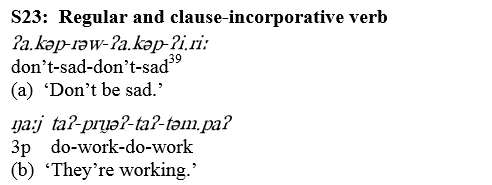
\includegraphics{Pacoh/src/PacohS23}

(이 문법서에서 하이픈은 형태morphs가 아니라 음운론적 어휘를 나타낸다. 하지만 포함된 형태들의 지분을 명확히 하기 위해 이 subsection에서는 전사의 `형태morphs'와 행간 주석이 하이픈으로 표시된 대로 대응된다.)

`슬프다'의 중첩어 rəw-ʔi.riː 와 일반화된 명사 `(구체적이지 않음) 일하다' prṵəʔ-təm.paʔ 가 분리되었고 비중첩어가 베껴졌다.

중첩의 시작점은 문장의 동사나 주어일 수 있는데 주어인 경우 완전한 문장 중첩이 일어나게 된다. 운율론적 음보를 유사한 패턴(analogical pattern)의 기본으로 사용한다. S24는 입력 어휘(input)에서 명사에 3개의 운율론적 음보가 연속되는 유사한 세트(analogical set)이다. 

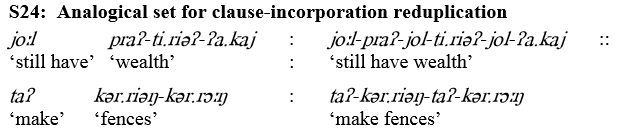
\includegraphics{Pacoh/src/PacohS24.png}

\subsubsection{전음절과 견본 중첩}
일음절 동사를 중첩한 다음 가운데에 [ʔi]를 추가한다. 만들어지는 동사는 자동사이고 행위의 의미적 일반성(generality)에 집중한다. 늘 자동사라는 사실은 의미적 일반화의 한 부분이기도 하다.

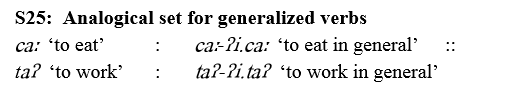
\includegraphics{Pacoh/src/PacohS25.png}

`~하는 척 하다'라는 의미를 갖는 중첩형은 taʔ `하다' $+$ 후행 자음과 조음점이 같은 비음 음절 $+$ 중첩동사의 1음절 $+$ 전음절 [ʔi-] $+$ 중첩 동사의 2음절

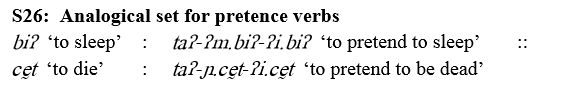
\includegraphics{Pacoh/src/PacohS26.png}

온점은 음절의 연결, 하이픈은 음보/음운론적 단어의 연결을 나타낸다.

\subsubsection{견본 중첩}
견본 중첩(template reduplication)은 1-2음절의 음운론적 단어 전체를 수반한다. 1음절은 2음절로, 2음절은 4음절로 일관적으로 일어나며
음절 구조도 일관된다. 일부 분절음의 교체가 일어나기도 한다.(2.5.3)

동사와 파생적으로 연결된 중첩형은 의미적으로 특수화를 거친다. 결과는 예측 가능하지 않을 때가 많다. 

명사의 중첩에서는 해당 명사를 포괄하는 일반적인 부류를 가리키는 말이 될 때가 많다. 이렇게 일반화된 명사도 상술한 절 결합적 어휘 형성에 음운론적 소재를 제공할 수 있다.

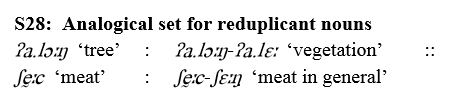
\includegraphics{Pacoh/src/PacohS28.png}

\section{기본 구 구조 개괄}
\subsection{기본 문장 구조}
주어가 동사에 선행하고 목적어는 동사를 후행한다.

특기할 만한 문제는 
\begin{itemize}
\item 주어 없는 문장
\item 목적어의 주제 부각 (전진) (일부 경우에 중간태로도 볼 수 있는)
\item 위치/시간 구와 의문사/의문사 구의 변이적인 위치 등이 있다.
\end{itemize}

전체적으로, 빠꼬어는 주제·논평(topic-comment) 구조 언어로 보는 것이 합당하다. 분명한 중간태의 사용 등 그런 통사적 유형에서 보일 만한 어순이 있다.

\begin{itemize}
\item 빠꼬어는 SVO 언어이다. S29에서 명령문은 대명사 주어를 갖지만 하위 절(the lower clause)은 갖지 않는다.

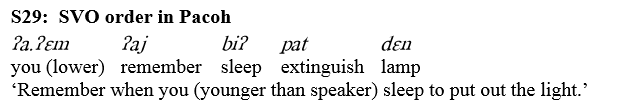
\includegraphics{Pacoh/src/PacohS29.png}

\item 주어는 자주 쓰이지만 적절한 담화적 맥락이나 특정 동사(10.5 비인칭동사 등)에서는 생략 가능하다.

\item 주제·논평 언어인 빠꼬어에서는 주제화된 구조에서 목적어가 문장 앞에 나오는 경우가 있다. 좀더 타동사적인 동사의 목적어가 주로 그렇게 된다. 주어, 장소 표현, 또 그 외의 논항 보어도 문장 앞에 나올 수 있다. 주제화는 ʔn.nɛh `이'나 kiː `그' 같은 어휘적 표지와 함께 일어날 수도 있지만 없이 일어날 수도 있다.  9.4 참조
\item 등식 관계(equational construction)에서는 계사(linking word)가 나올 수도, 나오지 않을 수도 있다. 이때 계사는 주어와 술어를 연결한다기보다는 주제와 논평을 연결한다. 9.4 참조

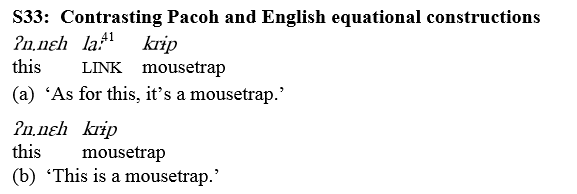
\includegraphics{Pacoh/src/PacohS33.png}

laː는 베트남어 차용어이다.
\item 일종의 중간태가 있는 것 같은 예시가 있다. 빠꼬어에 진정한 수동태 표지는 없다.

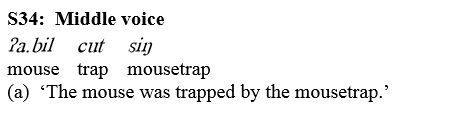
\includegraphics{Pacoh/src/PacohS34-1.png}

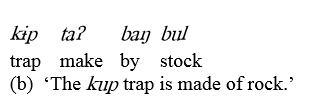
\includegraphics{Pacoh/src/PacohS34-2.png}

\item 부정에는 동사 부정과 명사 부정이 있다. 11.6참조
\item 비교급은 비교급 전치사를 쓰기도 쓰지 않기도 한다. 최상급을 나타내는 어휘는 따로 없다. 8.2 참조
\item 강조는 `사실인'이라는 단어와 동음인 lɨː `매우'로 나타낸다. 주로 후치 수식하지만 전치 수식도 가능하다. 상태 동사를 주로 수식하지만 행위 동사도 강조할 수 있다.
\item 위치와 시간 구는 문장 양쪽 끝 중 어느 쪽이든 유동적으로 위치할 수 있다.
\item 의문사의 분포는 베트남어의 영향으로 복잡하다. 앞으로 갈 수도 있고 (베트남어의 영향으로) 해당 격 위치에 나올 수도 있다. 7.3.2. 참조
\item 긍정-부정 질문, 기분, 명령조는 문장 말의 소사로 나타낼 수 있다. 9 참조
\end{itemize}

\subsection{복합적인 문장 구조}
독립절이 복합절 구문으로 결합할 때 접속사나 절 연결 부사와 같은 어휘에 의한 명시적인 표지는 나타날 수도 아닐 수도 있다. 명시적인 어휘 표지가 있는 복합 문장은 명확히 식별되지만 그렇지 않은 문장은 억양이나 의미적 맥락으로 식별한다. 그러한 복합절 구문은 하나의 억양 단위를 갖고, 절 하나만 가지고는 담화 맥락에서 의미적으로 불완전하다.

\begin{itemize}
\item 조건을 나타내는 어휘 nam `만약'은 사용될 수도 사용되지 않을 수도 있다. laː와 같은 절 연결 문장 소사가 쓰일 수도 있다. 9.3, 9.4 참조
\item 대조는 암시할 수도 있지만 보통 접속사 maː `그러나'(다른 소수민족 언어에서도 나타나는 베트남어 차용어)로 나타낸다.
\item 복합절 구조에서 시간 연속은 종종 어휘적으로 표시되지 않는다. (`S가 V1하고 V2한다'가 그냥 `SV1V2'로 나타난다는 뜻.) ɟəː `-한 뒤에' 같은 추가적인 절 연결 어휘가 사용될 수는 있다.
\item 목적은 주로 연속적으로 나타난다. (V1V2 하면 `V2하기 위해 V1한다'가 될 수 있다는 뜻.) 두번째 동사는 보통 표시되지 않지만 ɟo̰ːn `-하기 위해'가 쓰일 수 있다.
\end {itemize}

\subsection{명사구 구조}
일반적으로는 수식어-피수식어 구조이다. 좀더 자의적인 뭔가 다른 규칙을 따르기도 한다.
(기본 순서 수사-단위-명사-관계사-형용사-대명사-지시사)

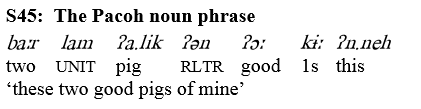
\includegraphics{Pacoh/src/PacohS45.png}


\begin{itemize}
\item mo̰ːj `각각의'나 ŋɛʔ `모든' 과 같은 범위 명사는 어떤 명사 하위부류든 선행할 수 있다.
\item 수사는 종별사와 함께 쓰여야 한다.
\item 종별사는 그에 대응하는 의미적 범주 안의 불가산 보통 명사와 쓰여야 한다. (종별사를 `가산명사', 종별사를 뒤따르는 명사를 `불가산 명사'로 부르고 있음)
\item 보통 명사 다음에 기술적인 상태 동사, 형용사 구, 소유 대명사, 지시사가 온다.
\item 가산 명사도 이상의 통사적 슬롯을 취하고 유사하게 수식될 수 있다.
\end{itemize}

\subsection{명사 간의 관계 표현: 전치사와 관계 명사}
시공간적 위치와 방향은 전치사(8장 참조)나 관계 명사(7.5 참조)로 나타낸다. 전치사와 관계 명사 사이에는 분포 상, 기능 상의 겹침이 있지만 구분할 이유가 몇 가지 있다.
\begin{itemize}
\item 가장 주요한 이유는 관계 명사가 비술어적 부가사(non-predicational adjunct)인 전치사와는 다르게 문장의 주어/주제 또는 술어/보어로 기능할 수 있다는 것이다.
\item 위치 전치사는 향격적(allative)이어서 S51(a)에서처럼 방향을 나타내지만 관계 명사는 고정적(static)이어서 S52(a)에서처럼 기본적으로 이양 불가능하게 소유된 위치를 표현한다.
\item 전치사는 S51(b)에서처럼 비교를 나타내는 등 좀 더 문법화되어 있고 의미적으로 추상적이지만 관계 명사는 S52(b)에서처럼 소유를 나타낸다.
\item 그 외에 역사적으로 관계 명사는 명사에서, 전치사는 동사에서 파생된 경우가 많다. 예를 들어 여격 전치사 ɟo̰ːn 은 동음의 동사 `주다'에서 파생되었을 가능성이 높은 반면 (이는 동아시아 및 동남 아시아에서 매우 보편적인 문법화 연속변이cline이다.) 여격 관계 명사 ʔa.dɔː 는 동음의 여격 대명사 `그의'와 관계되어 있다.
\end{itemize}

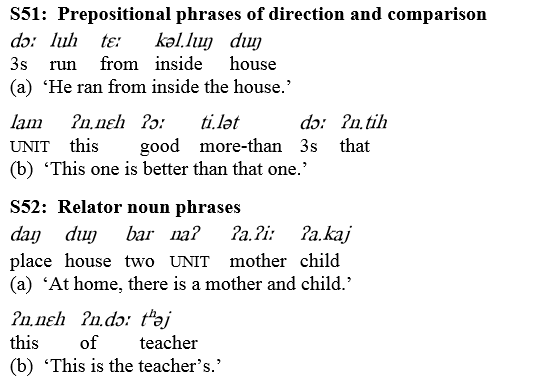
\includegraphics{Pacoh/src/PacohS51.png}


\section{부사}
부사는 선행하는 동사나 주어적 술어 또는 전치사적 술어를 의미 영역으로 취하는 동사 뒤의 요소이다.
부사가 표현하거나 수식하는 대상에는 다섯 종류가 있다.
\begin{enumerate}
\item 태도(manner, 의문 포함)
\item 강도
\item 결과
\item 동시적인 행위
\item 동시적인 상태
\end{enumerate}

일반적인 태도나 결과 부사는 가설적으로 열린 집합이지만, 강도, 의문, 동시 부사의 수는 한정적이다.

일부 부사는 대응하는 동음의 동사 형태가 있다. S53(a)에서 hoːj1은 상태 동사이고 해당 절의 술부 중심이지만, S53(b)에서 hoːj2는 강조 부사이다. 부사 hoːj2는 S53(b)에서 앞에 위치할 수 없고(cannot be preposed), 별개 동사로 해석하는 것은 다른 해석을 낳는다. 즉 `He tells stories, and he is very capable'이 아니다.)

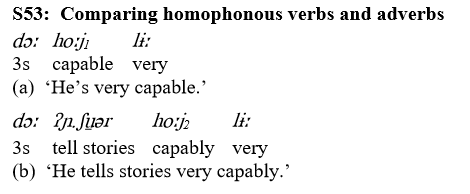
\includegraphics{Pacoh/src/PacohS53.png}

부사의 본질적인 특징으로 인해 liəh `again'과 같이 동사를 보어로 취하는 동사들은 부사로 볼 수 없다. 주어를 대체하는 전음절 [ʔu-]를 취할 수 있기 때문이다.

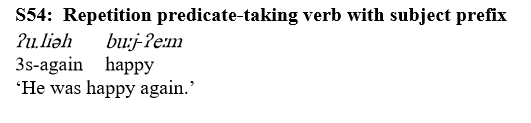
\includegraphics{Pacoh/src/PacohS54.png}

\subsection{일반 부사}
\omission

\subsection{강조 부사}
\omission

\subsection{의문 부사(`어떻게'와 `왜')}
\omission

\subsection{결과 부사}
\omission
%얘는 쓸까?

\subsection{동시 부사}
\omission

\section{접속사}
어휘적인 표지 없이 병렬하는 것이 빠꼬어에서는 흔하지만 몇 가지 접속사가 가, 교체, 대조를 나타내기 위해 쓰인다. 접속사는 연결짓는 대상에 따라 동시 발생에 제약이 생긴다.

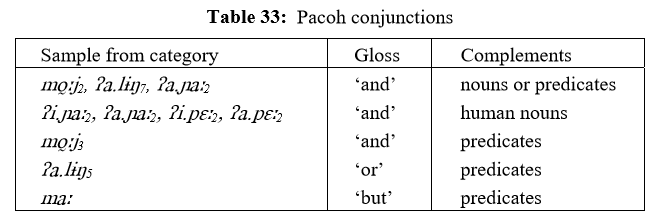
\includegraphics{Pacoh/src/PacohTable33.png}

\subsection{첨가 접속사 (`and')}
명사를 술어가 아니라 주어나 목적어로서 연결짓는다. ʔa.lɨŋ 은 `with'이라는 전치사와 동음이다. 이 전치사는 보통 주어에만 함께 쓰이지만, 접속사는 주어나 목적어에 좀더 자유롭게 나타날 수 있다.
S69, 70, 71 \omission

\subsection{인칭 접속사 (`and')}
인칭 접속사는 보어로 인간 명사만을 취한다. 이 종류에 속하는 모든 접속사가 빠꼬어의 이음절 대명사와 동음이고, 관계된 형태와 의미 자질을 공유한다.
이 접속사들은 2인칭이나 3인칭인 둘 이상의 보어를 취한다.

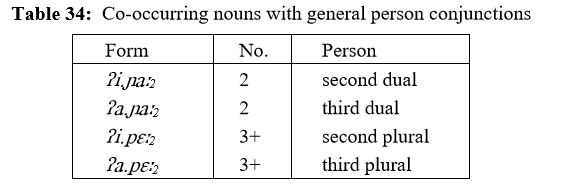
\includegraphics{Pacoh/src/PacohTable34.png}

이상의 형태는 단수 명사와 의미적으로 복수인 명사의 조합도 취할 수 있다. 이는 수와 인칭 요인의 의미적 일치이다. 보어에게 요구되는 자질은 동음의 대명사 형태의 자질과 일치한다. S. Watson (1964)

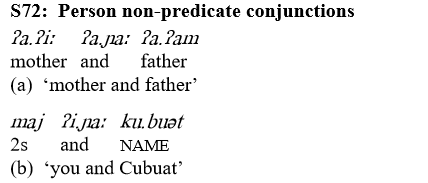
\includegraphics{Pacoh/src/PacohS72.png}

97년에 16세에서 20세 사이의 빠꼬 화자들로부터 채록한 자료에서는 ʔa.ɲaː가 명사의 인격성이나 보어의 수에 대한 고려 없이 쓰였다. S73에서 이 접속사는 사람이 아닌 보어를 취하고 있고 S74에서는 2개의 복수 보어를 취하고 있다. 여기에서 이 접속사는 비인격 비술어 접속사(non-person non-predicate-taking conjunction)로 여겨지는 것이다. 이것이 지역적 변이로 밝혀지지 않는다면, Watson이 기술한 접속사 패러다임은 소실되어가는 중일 수 있고 ʔa.ɲaː는 표준 기본형 접속사가 되어가고 있다.

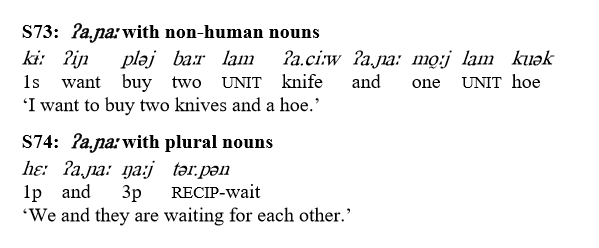
\includegraphics{Pacoh/src/PacohS73.png}

\subsection{술부를 취하는 첨가 접속사(`and')}
동사를 이을 때는 병렬이 흔하지만 특히 두 동사가 연속적이라기보다 동시적일 때는 접속사 mo̰ːj가 가끔 쓰인다.

\subsection{대체 접속사(`or')}
\omission

\subsection{대조 접속사(`but')}
빠꼬어의 유일한 대조 연장 접속사(contrary extension conjunction)는 maː `but'이다. 주로 두 동사 사이에 오지만 명사 술어도 취할 수 있다.